\documentclass{amsart}
\usepackage{graphicx}
\graphicspath{{./}}
\usepackage{hyperref}
\usepackage{csvsimple}
\usepackage{longtable}
\usepackage{lscape}
\usepackage{epigraph}
\title{Unpopularity of Politics}
\author{Zulfikar Moinuddin Ahmed}
\date{\today}
\begin{document}
\maketitle

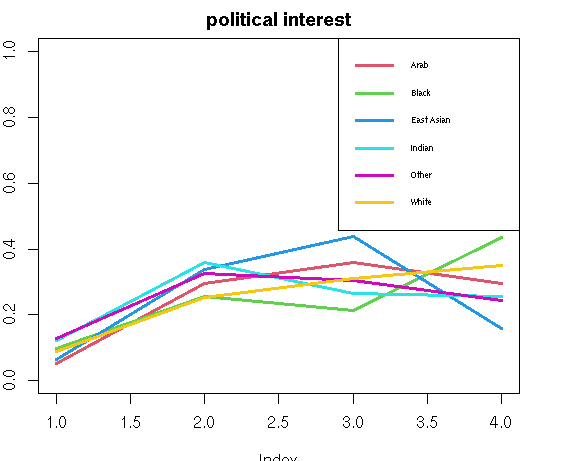
\includegraphics[scale=0.8]{politics.png}

% latex table generated in R 4.0.3 by xtable 1.8-4 package
% Sat May 15 05:44:39 2021
\begin{table}[ht]
\centering
\begin{tabular}{rr}
  \hline
 & People not interested in politics \\ 
  \hline
Arab & 0.65 \\ 
  Black & 0.65 \\ 
  East Asian & 0.60 \\ 
  Indian & 0.52 \\ 
  Other & 0.55 \\ 
  White & 0.66 \\ 
   \hline
\end{tabular}
\end{table}

The mean $\mu=0.60$ with $\sigma=0.059$.  This is a beautiful ethnicity independent result.  

\section{Tight Bounds on Interested People}

For 'very interested' we have mean 0.092 and standard deviation 0.03.  For 'somewhat interested' mean 0.304 and standard deviation 0.044.  These are remarkably tight bounds.  There is more variance on the difference in 'not interested' and 'not interested at all'.

These are extremely nontrivial regularities that are global and ethnicity-independent.

\section{Wider Ethnic Differences in Confidence in Government}

While interest in politics follows tight uniformity independent of ethnicities, there are stronger ethnicity effects in {\em Confidence} in government.  These are delicate differences that require a bit of care.


\end{document}